\subsection*{Ještěrky} % (fold)
\label{sub:ještěrky}

\begin{multicols}{2}


Tábor jsme si jako Ještěrky moc užily. Snad poprvé v historii jsme se tam sešly všechny. Vychutnávaly jsme si chvilky v přírodě. Konečně se nám zase podařilo uniknout pryč od toho pražskýho stereotypu a městskýho života. Moc ráda budu vzpomínat např. na klidné manévry s mojí etapkovou skupinou. Z Ještěrek jsem byla s Olivou a E.T. a moc jsme si užily společný čas. Jediné, co by celkovému dojmu z tábora snad ještě přidalo, by byl blýzký potok. Mohu potvrdit z vlastní zkušenosti, že tekoucí voda z pumpy se nedá s proudem chladivého potaka či říčky vůbec srovnávat. Avšak i přes tento malicherný nedostatek jsou mé pocity ohledně prázdnin strávených na táboře kladné.
\podpis{Viki}


Pro mě byly velmi příjemné relaxační akce, už jen z toho důvodu, že tyto programy obsahovaly všechno, jen ne práci a nepohodu.
Ale co to vlastně takova relaxační akce je? 
Když bylo moc velké horko, a když říkám velké, myslím tím ultra mega velké, tak nám vedoucí řekli, ať si vezmeme plavky, ručník a všechny potřebné věci k pohodě u vody a buď jsme pochodovali na vlak, abychom se přiblížili k daleké řece, nebo jsme šli k ne tak dalekému rybníku.
Po doražení na místo činu jsme jedli, pili, koupali se, radovali se, hráli hry, masírovali se a dělaly všechny ty nádherné činnosti, které se dělají, když je léto a dobrá nálada.
Za tábor jsme tyto rajské chvíle mohly zažít dvakrát.
A na konec mám takové malé ponaučení: 
Děti, když jedete ven v létě relaxovat k rybníku či řece, vždy se mažte opalovavím krémem!
Slunce je zprvu příjemné a dobrý služebník, ale také dokáže být zlý pán. Ano, nikdy si nepřejte vědět, jaké to je mít spálenou, loupající se hroší kůži. :)
\podpis{Jogurt}

To bylo zase jednou na táboře. Přesněji řečeno na začátku tábora. A nebo taky na konci stavebky. To záleží na úhlu pohledu. Ale to už je jedno. Prostě přijížděli mladší členové a starší jim šli naproti na vlakovou stanici. A tak se na vlakové stanici všichni sešli i s batohy obsahujícími spacáky a věci na bivak a ještě spolu s divně oblečeným Wexlákem a Kibitzem. Ti nám oznámili, že jsme poutníci, a proto si musíme vzít z batohů jen to nejnutnější a uvázat si to na kus prádelky, který každý dostal. Dále jsme byli rozděleni na dvě skupiny a dostali jsme slovní popis cesty. A u toho začal celý problém, protože Kibitzovo písmo se luští opravdu špatně. No, ale vyluštili jsme z něj, že máme jít na náves, zahnout po mostě a potom proti proudu řeky a kolem krav po loukách do lesa. Všechno šlo hladce až na malé zdržení, když mladší kluci plašili krávy. Jenže potom nám začal popis cesty neodpovídat naš
í reálné cestě. Šli jsme po vykácené mýtině a po silničce mezi poli. Řeku jsme úplně ztratili. Až jsme dorazili opět do Ostrovce, tedy vesnice, ze které jsme vyráželi. Byli jsme unavení a doufali jsme, že už je třeba tak pozdě, že nás Kibitz už nikam nepošle, ale řekne, že se můžeme vrátit do tábora. To se však nestalo a Kibitz nás poslal zpět na vlakovou stanici, abychom začli znova. Tentokrát mi ale řekl barvy cest, po kterých máme jít. Napodruhé se cesta odehrávala bez zbytečných přestávek (kluci byli dokonce tak unavení, že i krávy přešli bez povšimnutí). No a dál už si to bohužel moc nepamatuji. Myslím, že jsme došli někam, kde jsme se setkali s druhou skupinkou a společně jsme pak šli na nějaký hrad (taky jsme se ještě stihli ztratit), kde byl Wexlák a Kibitz a večeře. Potom myslím Kibitze někdo unesl a všichni jsme šli s Wexlákem spát někam do lesa. A druhý den jsme asi šli zase zpátky do tábora. Jo, myslím, že takhle nějak to bylo, ale omluvte prosím případné nepřesnosti. Závěrem bych jen chtěla varovat všechny skupinky, které budou mít někdy v budoucnu co do činění s Kibitzovým rukopisem, že se při luštění pěkně zapotí :-D.

\podpis{Huhma}


\end{multicols}

\begin{center}

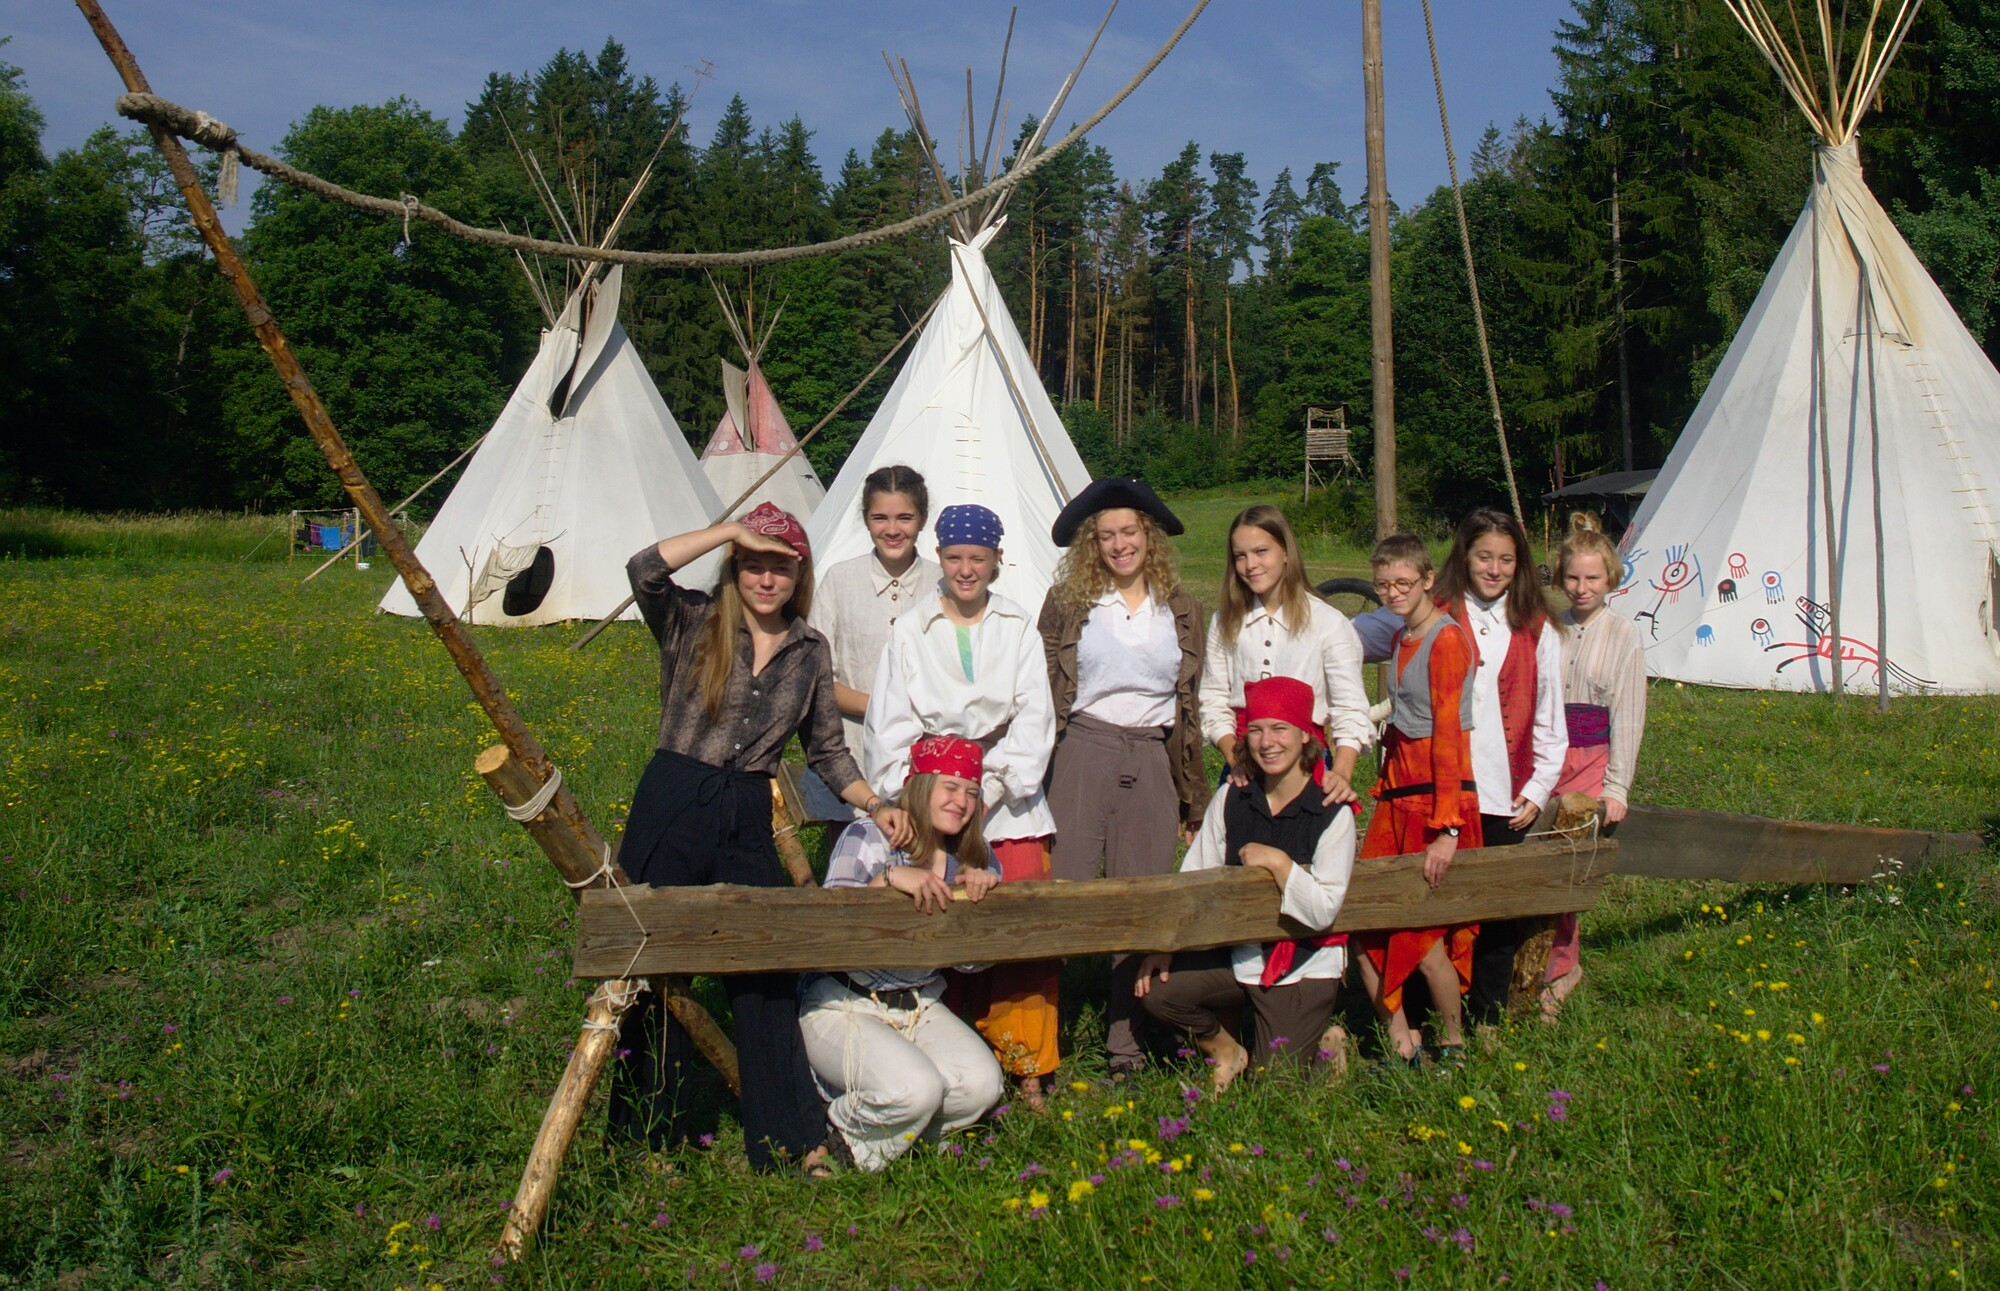
\includegraphics[width=10cm]{img/druziny/jesterky.jpg}

\end{center}


% subsection ještěrky (end)